\documentclass[12pt]{article}
        \usepackage{graphicx,type1cm,eso-pic,color}
        \usepackage{hyperref}
        \usepackage[left=3.0cm,right=3.0cm,top=2cm,bottom=2cm,headheight=13.6pt]{geometry}
        \usepackage{subfigure}

\makeatother


\title{Manual for HPS ECal v2.0}

\author{ECal On-Call Cell Phone: 757-810-1489 \\ 
Authors: \\
General contact: Rapha\"el \textsc{Dupr\'e} (\texttt{dupre@ipno.in2p3.fr})\\ 
LED system: Andrea \textsc{Celentano} (\texttt{andrea.celentano@ge.infn.it})\\
LV/HV/Chiller/Temps/Scalers: Nathan \textsc{Baltzell} (\texttt{baltzell@jlab.org})\\
}

\date{\today} %01/07/2014


\begin{document}
\maketitle{}

\tableofcontents

\newpage
   \section{General description of the ECal}


The electromagnetic calorimeter (ECal), installed downstream of the pair spectrometer dipole magnet (figure~\ref{GView}), performs two essential functions for the experiment: it provides the trigger signal and helps identify electrons and positrons. The ECal modules are based on tapered 160 mm long PbWO crystal with a 13.3x13.3 mm$^2$ (16x16 mm$^2$) front (rear) face wrapped in VM2000 multilayer polymer mirror film. The scintillation light, approximately 110 photons / MeV, is read out by a 10x10 mm$^2$ Hamamatsu S8664-1010 Avalanche Photodiode (APD) with 75\% quantum efficiency glued to the rear face surface. The low gain of APDs (150 pC/pC) is compensated with custom-made preamplifier boards, which provide a factor of 225 amplification of the APD signal. In front of the crystals, LEDs are installed to send light into the crystals. These are used in order to check the proper functioning of the ECal and provides complementary information to evaluate gain variations in the various channels of the calorimeter (see figure~\ref{AmplChain}).

\begin{figure}[htpb]\center
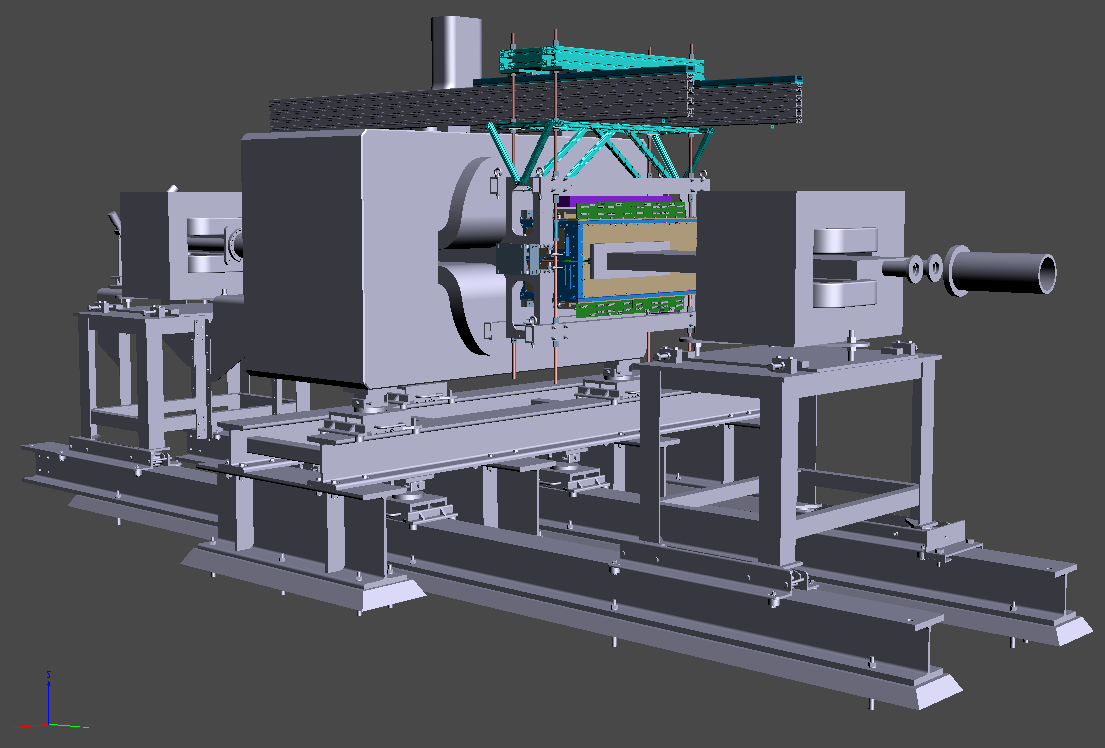
\includegraphics[width=0.75\textwidth]{pics/GView.png}
\caption{\label{GView} General view of the ECal (in color) suspended at the downstream end of the HPS analyzing magnet.}
\end{figure}
      
The ECal is built in two separate halves that are mirror reflections of one another relatively to the horizontal plane. The 221 modules in each half are supported by aluminum frames and arranged in rectangular formation with five layers and 46 crystals / layer, except for the layer closest to the beam where nine modules were removed to allow a larger opening for the outgoing electron and photon beams (figure~\ref{Crystals}). Each half is enclosed in a temperature controlled box ( $< 1^\circ$F stability and $< 4^\circ$F uniformity) to stabilize the crystal light yield and the operation of the APDs. Four printed circuit boards (referred as mother boards) mounted on the back plane penetrate the enclosure and are used to supply the $\pm5$ V operating voltage for the preamplifiers, the 400 V bias voltage to the APDs, and to read out signals from the APDs. Each half of the ECal is divided into 26 bias voltage groups formed in order to minimize the gain spread of the APD-preamplifier couples.

\begin{figure}[htpb]\center
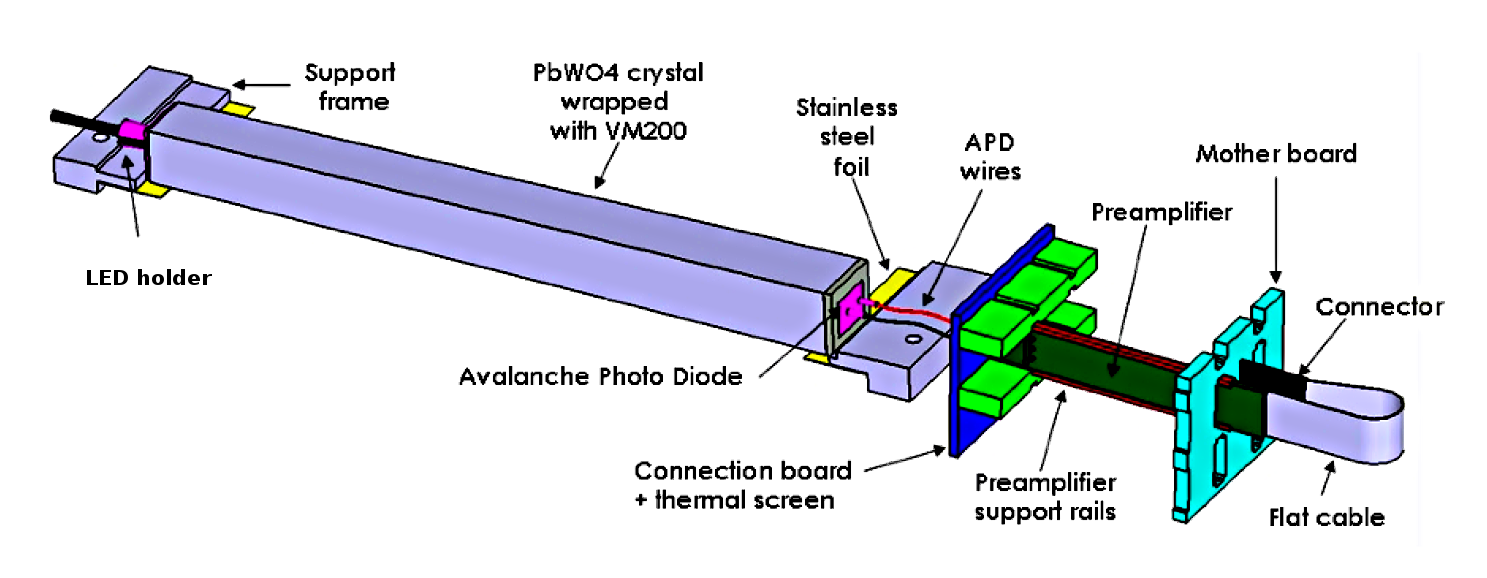
\includegraphics[width=0.75\textwidth]{pics/CrystalAssembly.png}
\caption{\label{AmplChain} View of an ECal crystal and the amplification chain.}
\end{figure}
After a 2:1 signal splitter, 1/3 of an amplified APD signal is fed to a single channel of a JLab flash ADC (FADC) board. 2/3 of the signal is sent to a discriminator module before a TDC for a time measurement. The FADC boards are high speed VXS modules digitizing up to 16 crystal signals at 250 MHz and storing 4 ns samples with 12-bit resolution. When a trigger is received, the pipeline is read on these boards from 5 samples before and 30 after the trigger time (those values will be adapted during commissioning).

\begin{figure}[htpb]\center
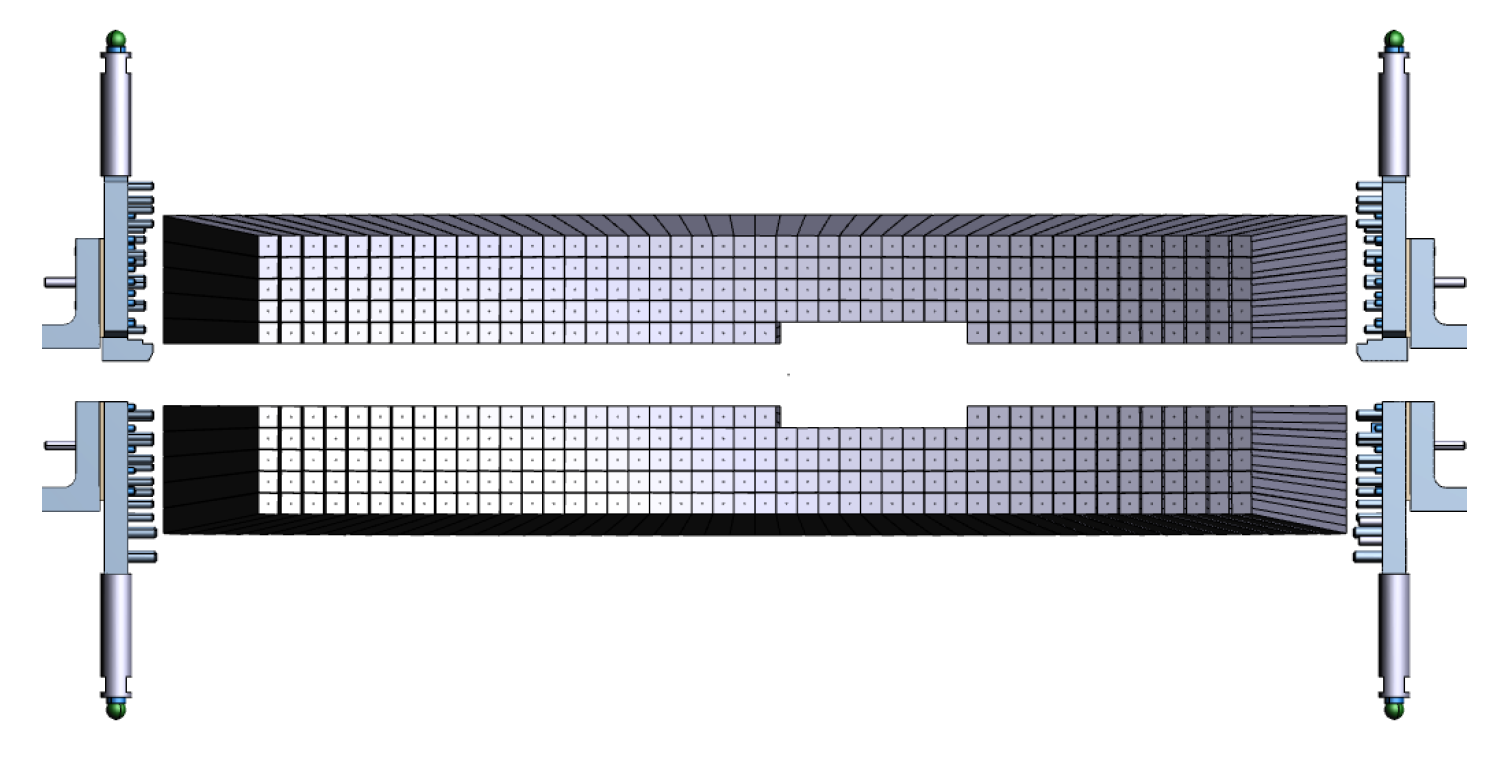
\includegraphics[width=0.75\textwidth]{pics/ECal2.png}
\caption{ \label{Crystals} Front view of the ECal crystals layout.}
\end{figure}

 \twocolumn
\part{Shift Takers Instructions}

\vspace*{\stretch{1}}      
All ECal controls are accessible through EPICS, from the main HPS\_EPICS window (figure~\ref{EPICSmain}).  If not already running, it can be opened by executing
the command \begin{center}\texttt{hps\_epics}\end{center} in a terminal on any of
the \texttt{clonpc\#\#} workstations in the Hall-B counting house.

{\em   All shift workers should be using user \texttt{hpsrun} for all instructions in this document.}

The primary ECal screen is shown in figure~\ref{fig:ecal_all} and opened via the {\bf ECAL} button in the right side of the main HPS EPICS screen (figure~\ref{EPICSmain}).

From the main HPS\_EPICS window you can also access individual screens with more controls and details, {\bf Temperature monitoring} in {\it Miscellaneous} then {\it ECal Temperature}, the {\bf ECal chiller} in {\it Devices} then {\it Chiller (ECAL)}, the {\bf Scalers} in {\it ECal Scaler GUI}, the {\bf ECal high voltage} in {\it Voltages} then {\it ECal HV} and the {\bf LED control panel} in {\it Devices} then {\it Flasher}.  


\vspace*{\stretch{1}}      

\begin{figure}[h!]
\center
%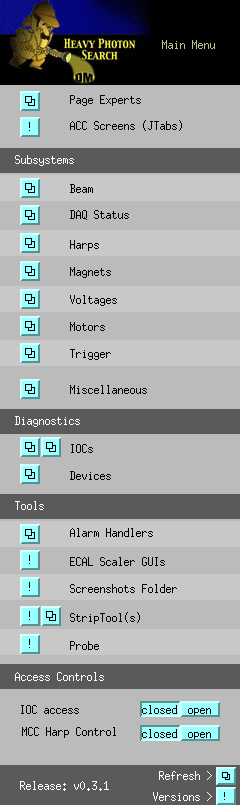
\includegraphics[width=0.38\textwidth]{pics/hps_epics_2014_12_15.png}
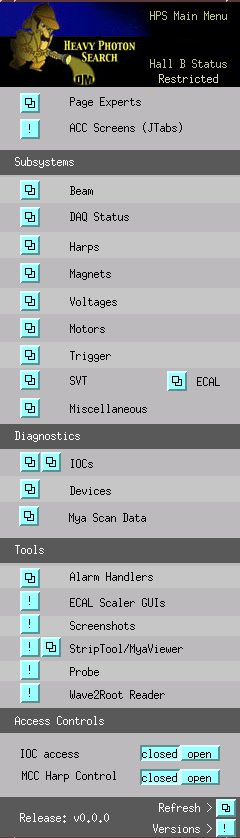
\includegraphics[width=0.38\textwidth]{pics/hps_epics_2015_09_18.png}
\caption{ \label{EPICSmain} View of the Hall-B EPICS main window.}
\end{figure}

 \onecolumn

 \section{Primary ECal EPICS Screen}
 This one screen combines all basic ECal EPICS controls and monitoring into one window.  It is accessible from the {\bf ECAL} button in figure~\ref{EPICSmain}.  This includes embedded versions of the dedicated screens in the following sections:  temperature sensors, chiller, and low and high voltage.  
 
 This screen provides the only ECal {\em controls} shift workers should need, which is to turn HV on and off via the red and green buttons.  However, this should be supplemented by the strip charts for temperature and HV current, as well as cctv webcams, for additional {\em monitoring} in the following sections.

The grey square buttons in the top right of each section of this main ECal screen provide
access to more detailed or expert screens for the corresponding subsystem.


\begin{figure}[htbp]\centering
    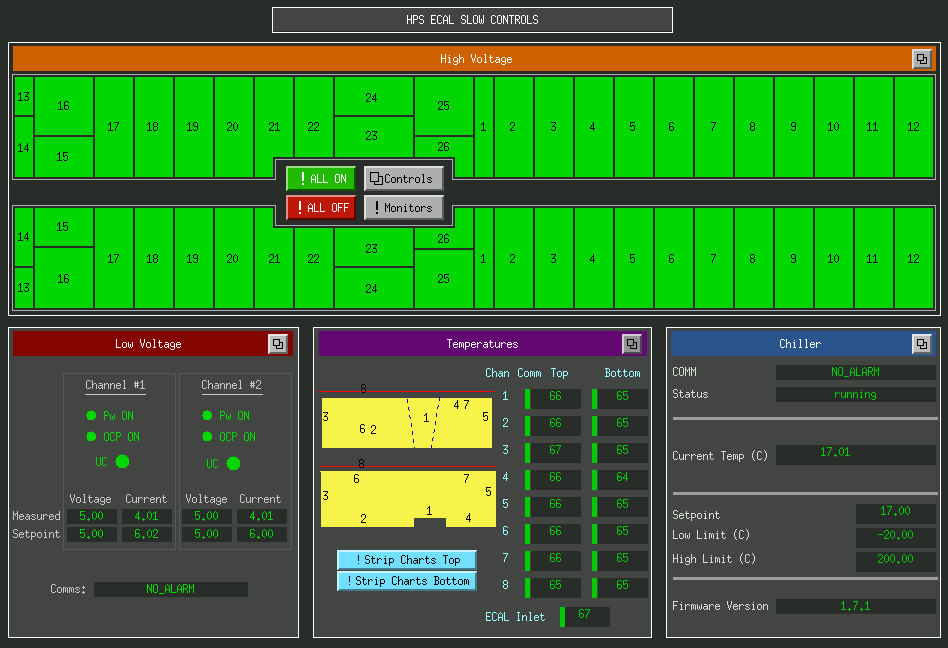
\includegraphics[width=15.5cm]{pics/epics_ecal_all.png}
    \caption{The primary EPICS screen needed for shift workers to monitor ECal.\label{fig:ecal_all}}
\end{figure}

\newpage
\section{Temperature}
The ECal temperature should remain as stable as possible in order to avoid gain variation in the system.  Cooling controls and monitoring are desribed in this section.

\subsection{Temperature Sensors}
Eighteen temperature sensors are placed in the ECal enclosure and should be monitored through ECal's main EPICS screen and the strip charts shown in in figure~\ref{temp2}. Variations of two degrees F or more during a shift should be reported to ECal expert on call and noted in the log book.  The strip charts are accessible from the two buttons in the temperature section of Figure ~\ref{fig:ecal_all} (and also the main HPS\_EPICS screen in Figure \ref{EPICSmain}).
%\begin{figure}[htbp]
%\center
%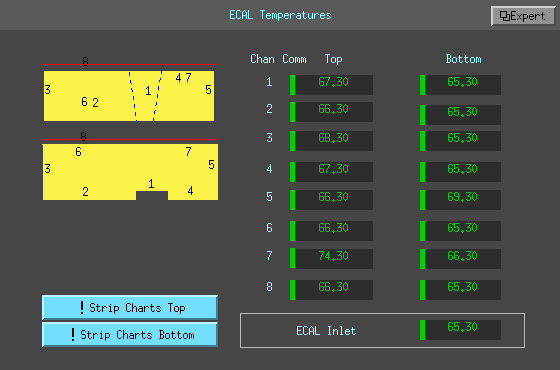
\includegraphics[width=0.5\textwidth]{pics/EcalTemp_2014_12_20.png}
%\caption{ \label{temp} View of the EPICS temperature monitoring window.}
%\end{figure}
\begin{figure}[htbp]
\center
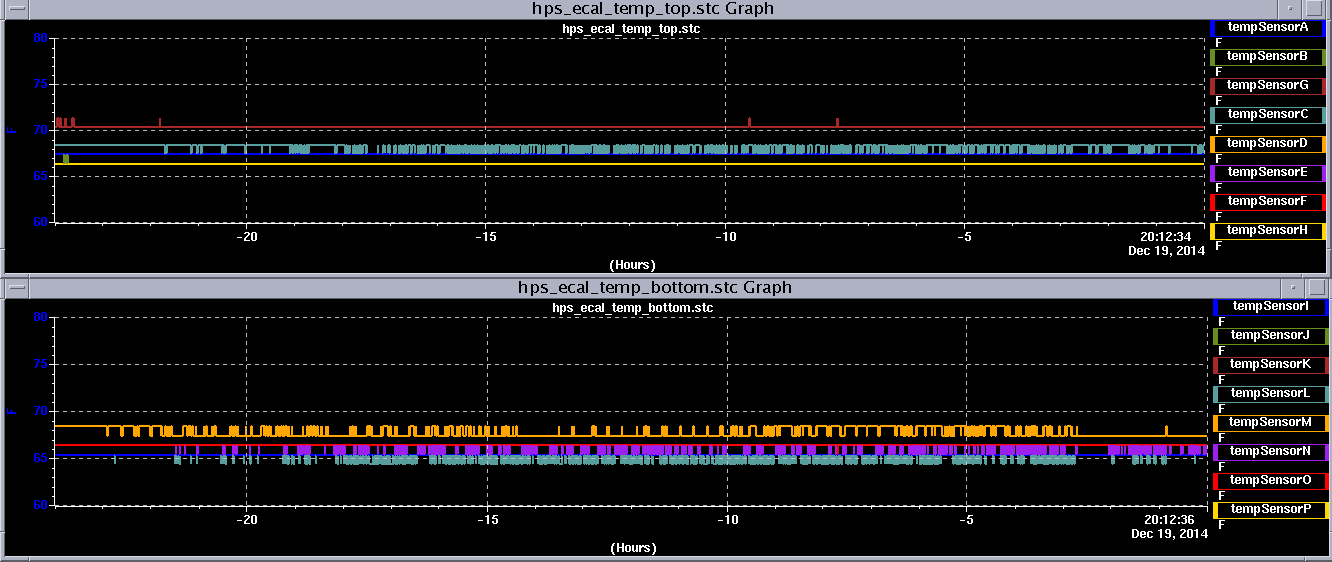
\includegraphics[width=0.45\textwidth,height=4.5cm]{pics/ECal_temp_s.png}
%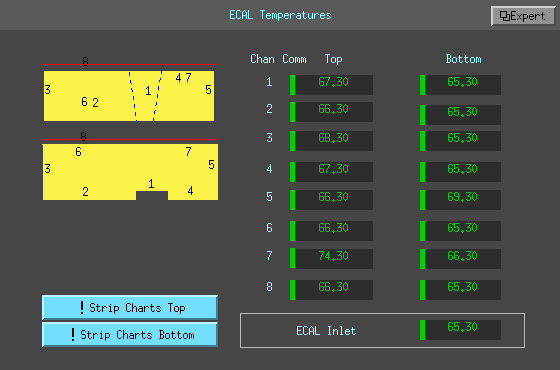
\includegraphics[width=0.39\textwidth]{pics/EcalTemp_2014_12_20.png}
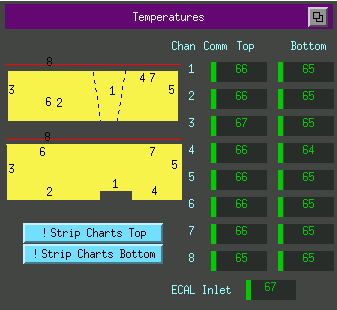
\includegraphics[width=0.3\textwidth,height=4.5cm]{pics/epics_ecal_temp.png}
\caption{\label{temp2} View of the EPICS temperature monitoring strip charts (left) and the temperature portion of the main ECal EPICS screen (right).}
\end{figure}

\subsection{Chiller}
         The chiller allows to keep the calorimeter at the right temperature and should be ON and set at 17C at all times. The chiller can be monitored through its webcam and EPICS controls (figure~\ref{ChillerCam}). Shift takers should not attempt to change the chiller settings and call ECal expert in case of problem.  The webcam is accessible in a web browser via the url \texttt{cctv10.jlab.org} and the ``Monitoring'' tab on the {\bf HPS Run Wiki}.

\begin{figure}[htbp]
\center
%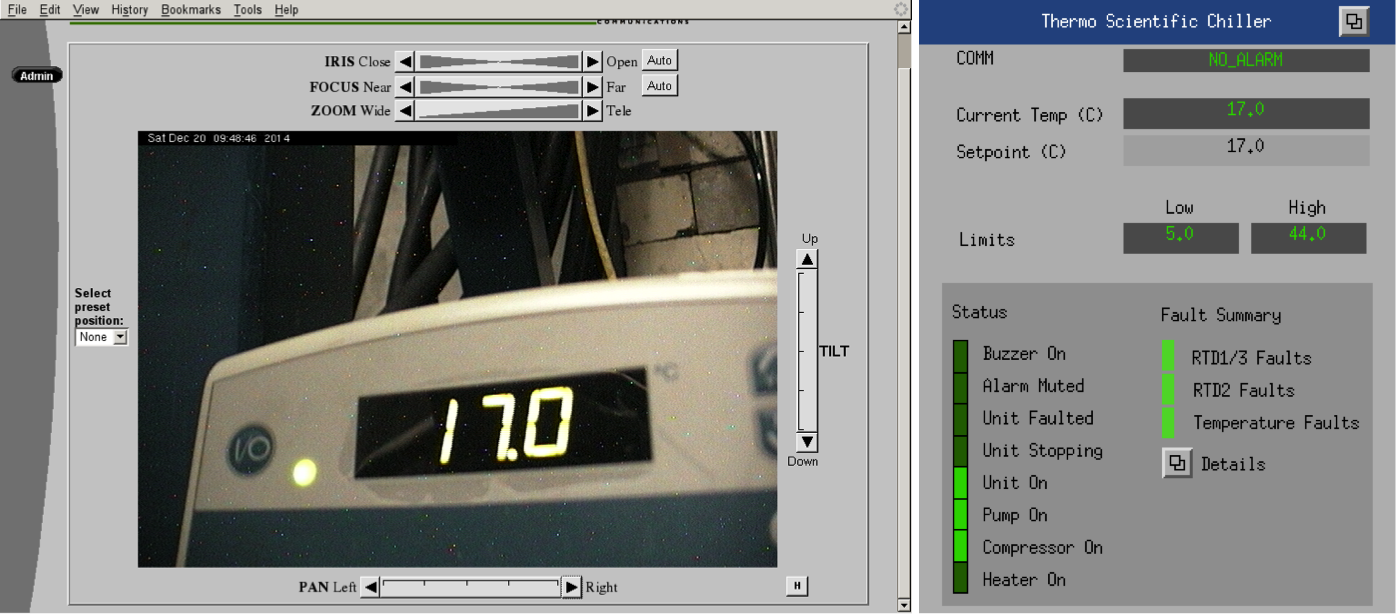
\includegraphics[width=0.99\textwidth]{pics/ChillerCombo.png}
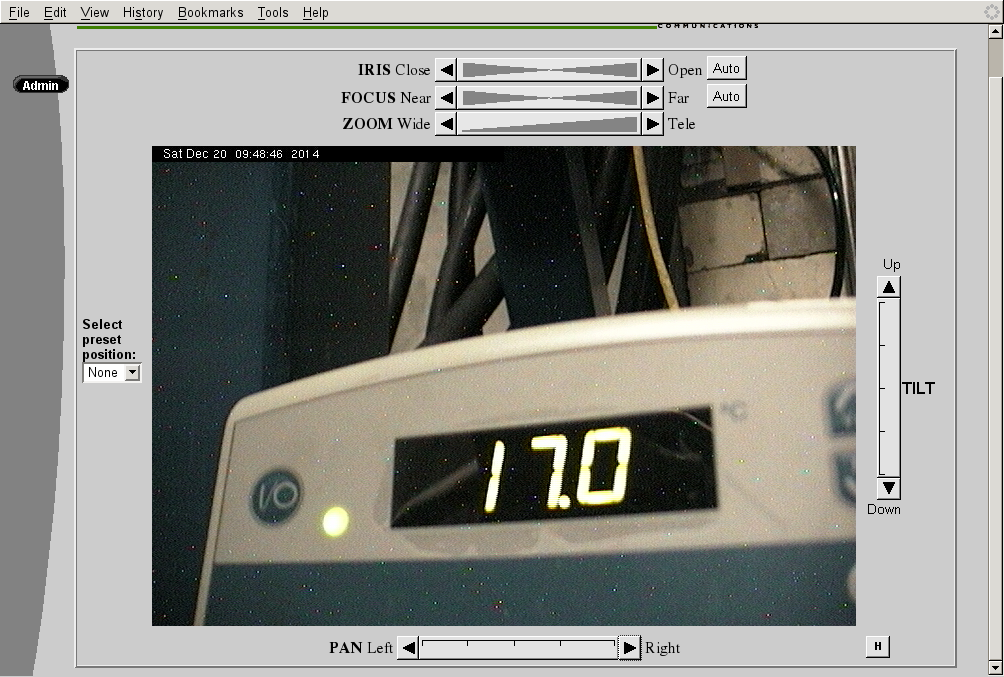
\includegraphics[width=0.45\textwidth,height=4.5cm]{pics/ChillerCam_2014_12_20.png}
%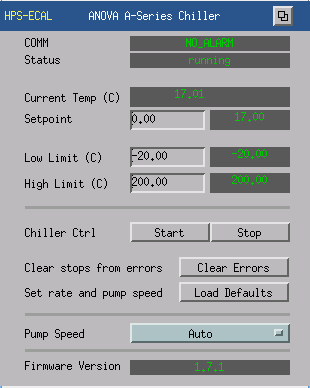
\includegraphics[width=0.3\textwidth,height=5.5cm]{pics/ChillerWin_2016_1_17.png}
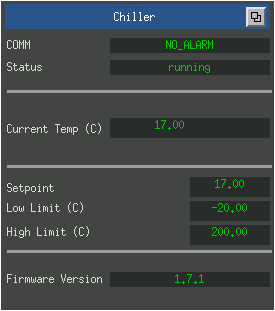
\includegraphics[width=0.3\textwidth,height=4.5cm]{pics/epics_ecal_chiller.png}
\caption{ \label{ChillerCam} View of the chiller's \texttt{cctv10.jlab.org} webcam (left) and its portion of the main ECal EPICS window (right).}
\end{figure}

\newpage

\section{Low Voltage}
{\em The low voltage power supply must be on before HV is turned on, and changing its settings requires contact with an ECal-expert.}
      
LV should be monitored using its webcam and its portion of the main ECAL EPICS screen (both shown in figure~\ref{LVCam}). Call the ECal expert if this appears not to be ON or shows an abnormal current for either of its two channels.  {\em Normal current is between 4.0 and 4.2 A for both channels}.  This webcam is accessible via the url \texttt{cctv11.jlab.org} in a web browser and the ``Monitoring'' tab on the main {\bf HPS Run Wiki}.
\begin{figure}[htbp]
\center
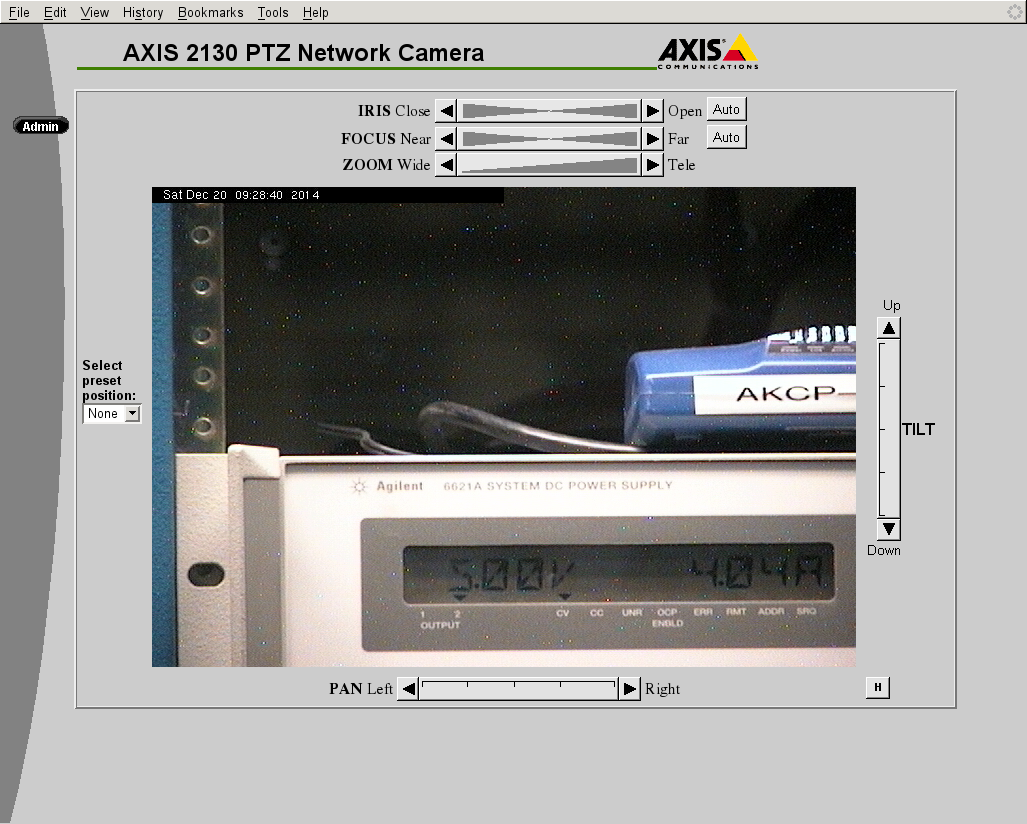
\includegraphics[width=0.49\textwidth,height=5.5cm]{pics/LVCam_2014_12_20.png}
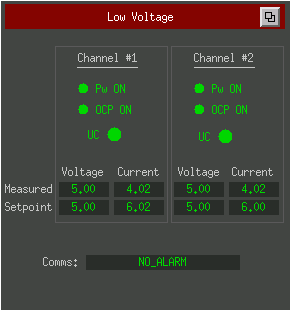
\includegraphics[width=0.39\textwidth,height=5.5cm]{pics/lvnovice.png}
\caption{ \label{LVCam} View of the LV suuply by webcam (\texttt{cctv11.jlab.org}) and its portion of the main ECAL EPICS screen.}
\end{figure}

\section{High Voltage}
      \subsection{Turning ON/OFF High Voltages}

      The high voltage supply of the ECal is controlled and monitored using the main ECal EPICS window (Figure ~\ref{fig:ecal_all}).  It has buttons to ramp up and down the entire calorimeter's high voltages (labeled ``ALL ON'' and ``ALL OFF''), open windows for individual channel control (figure~\ref{HVControl}), and open more detailed expert views (e.g. figure ~\ref{HV}).

   \subsection{HV Current Monitoring}
   Individual channels' currents can be monitoring in figure~\ref{HVControl}, and strip charts should be open for long term monitoring.  The strip charts are accessible from the main ECal screen (figure ~\ref{fig:ecal_all}) under the HV sections' ``Monitors'' button (and also from the HPS\_EPICS screen (figure~\ref{EPICSmain}) via the ``Strip-Tool'' button).  An example is shown in figure~\ref{fig:hvcurrentstrips}.  Jumps or drifts in current of more than 1 A should be noted in the logbook.

   \begin{figure}[htbp]\centering
       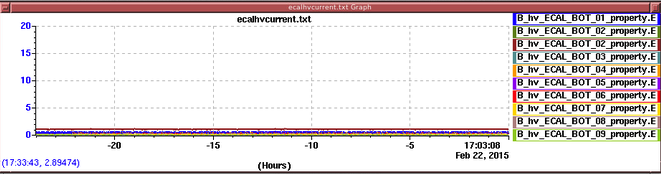
\includegraphics[width=16cm]{pics/hvcurrentstrip.png}
       \caption{HV Current strip charts.\label{fig:hvcurrentstrips}}
   \end{figure}


   \subsection{Responding to HV trips}

   HV problems, in particular trips, are indicated by a red group in the main ECal EPICS GUI (figure~\ref{fig:ecal_all}).  HV trips will also be announced by the alarm handler.  During normal operations with HV ON, there should be no red groups in Figure \ref{fig:ecal_all} and no ECAL HV alarms.  Contact the ECAL expert on-call in case of uncertainty.
     
In case of an HV trip, or a red region in Figure \ref{fig:ecal_all}:
\begin{itemize}
    \item Try to reenable the HV group by turning it back on in the EPICS HV control screen (figure~\ref{HVControl}) accessed via the ``Controls'' button in the main ECal EPICS screen (Figure \ref{fig:ecal_all}).  (An alternative is just pressing the ``ALL ON'' button in the 
main ECal EPICS screen, which will effectively turn all channels on.)
    \item Record the trip in the log book with precise indication of the group and run
        number concerned. 
\end{itemize}
      
      {\em Note, the HV can take up to 3 minutes to turn back on so you should end the current run and begin a new one when the high voltage is back on. If you cannot get a HV group to work contact the ECal expert on call.}

      {\bf If you encounter more than two HV trips during your shift for the same group, you should notify the ECal Expert.}

\begin{figure}[htbp]
\center
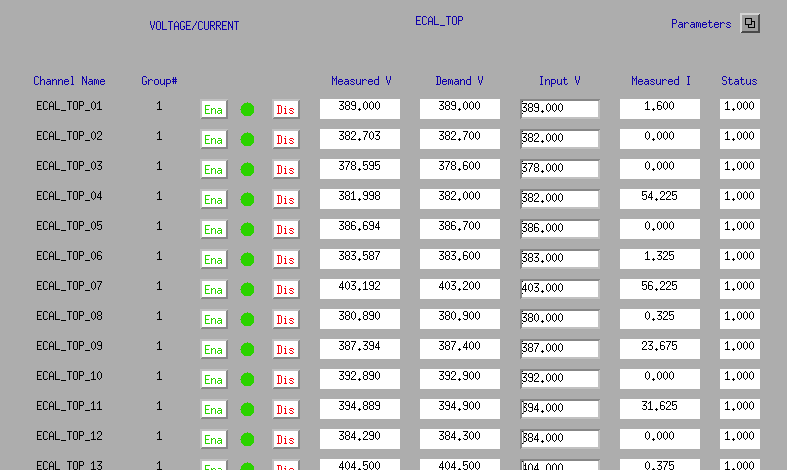
\includegraphics[width=0.85\textwidth]{pics/ecalhv_setting_2014_12_15-SUBSET.png}
\caption{ \label{HVControl} Cropped view of the EPICS ECal HV control window for individual channels.}
\end{figure}

\clearpage
\newpage
      \section{Scalers}

      Rates seen by the ECal are available in the ROOT-based GUI shown in Figure \ref{Scalers}, which represent the rates as seen by the FADC electronics.  This display is accessible via the main HPS\_EPICS window under the {\bf ECAL Scaler GUIs} button, and also by running \texttt{hps\_ecal\_scalers} in a terminal.  {\em As of 2016, the discriminators are disconnected and only the FADC rates are accessible.}
      
      One can also see clustering scalers from the DAQ ``diaggui'' screen (figure~\ref{DAQscalers}), accessible also by the {\bf ECAL Scaler GUIs} button or by executing \texttt{diaggui.sh} in a terminal.  This GUI indicates the rates of clusters reconstructed by the trigger electronics. 
      
      These numbers should all remain constant within $^\sim10\%$ during stable beam operation. A strong increase is the indication of bad beam conditions or the presence of a new source of noise in the ECal system.  If the latter case, please contact ECal expert on call.
\begin{figure}[htbp]
\center
%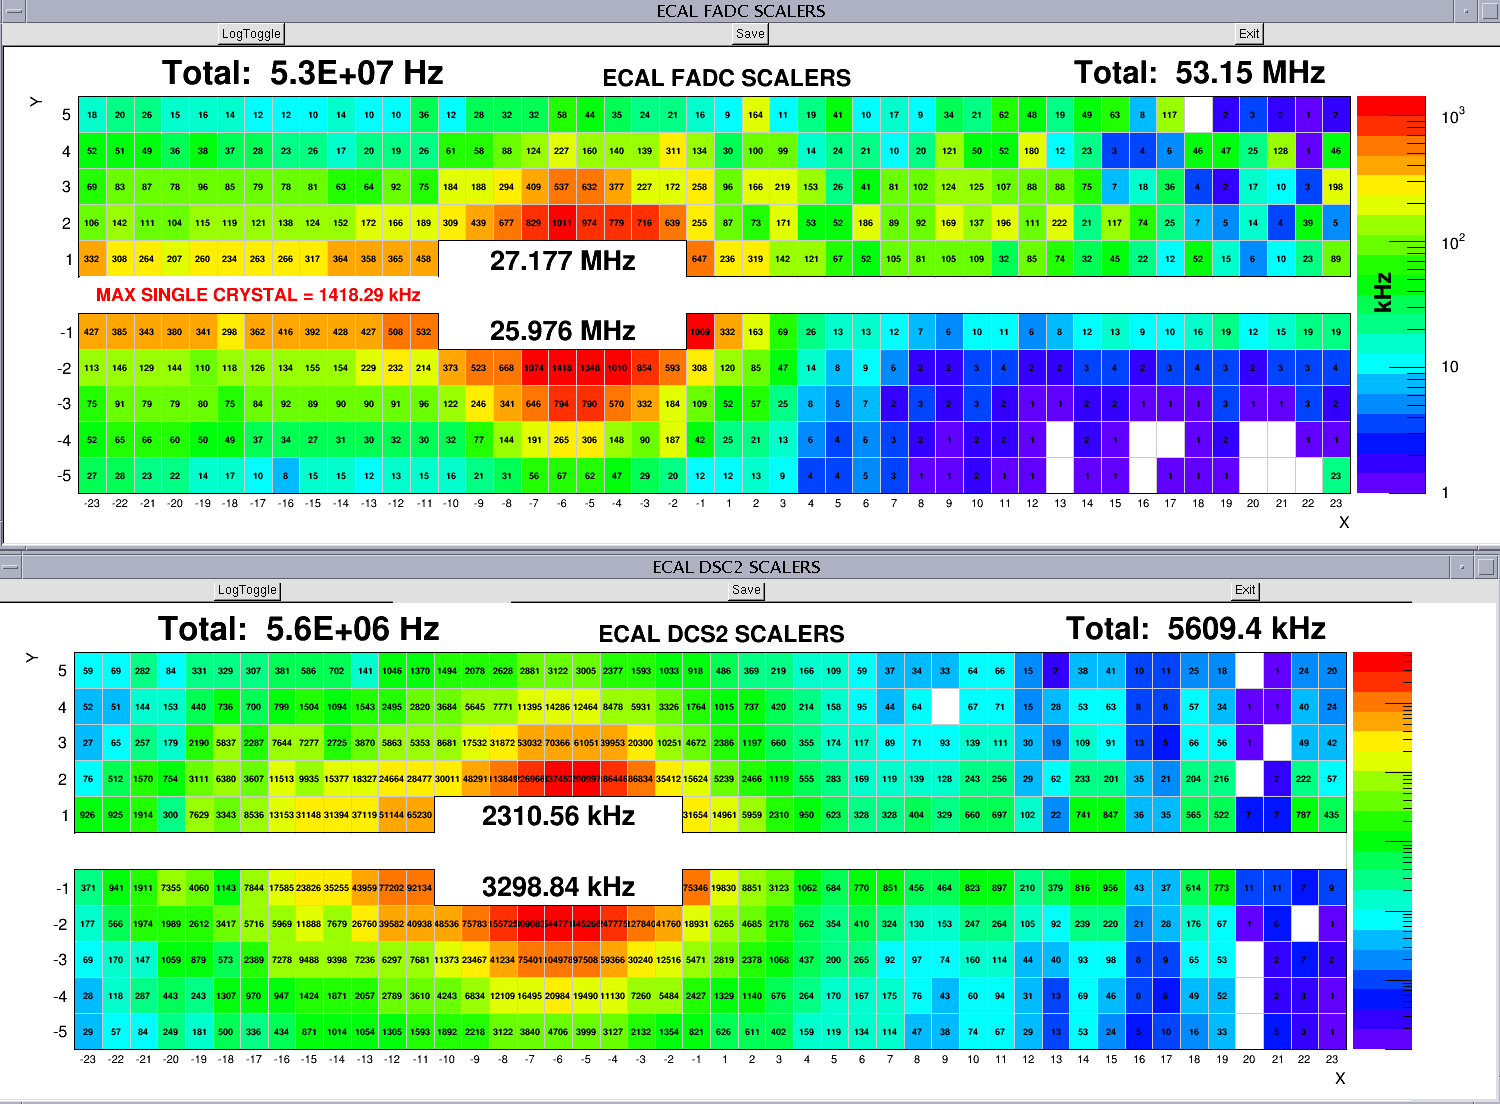
\includegraphics[width=0.75\textwidth]{pics/ECAL_FADC_SCALER_2014_12_20.png}
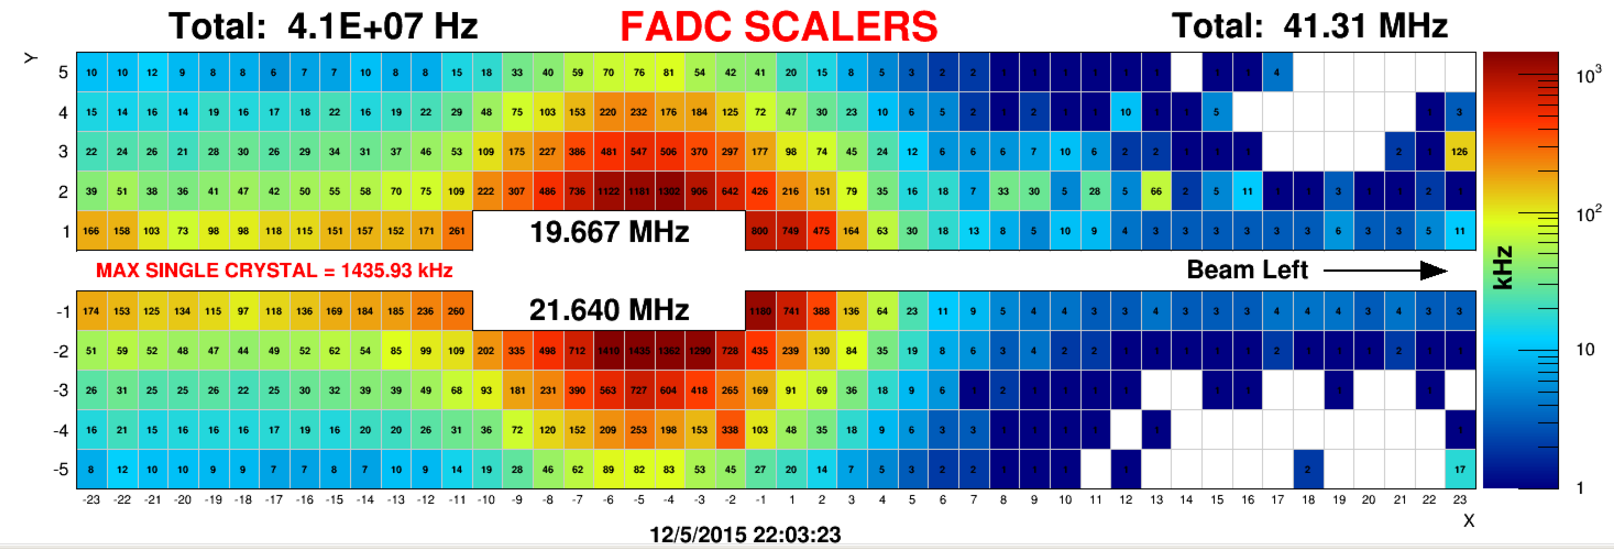
\includegraphics[width=0.9\textwidth]{pics/fadcscalers_2015run.png}
\caption{ \label{Scalers} View of the EPICS FADC scalers window.}
\end{figure}
\begin{figure}[htbp]
\center
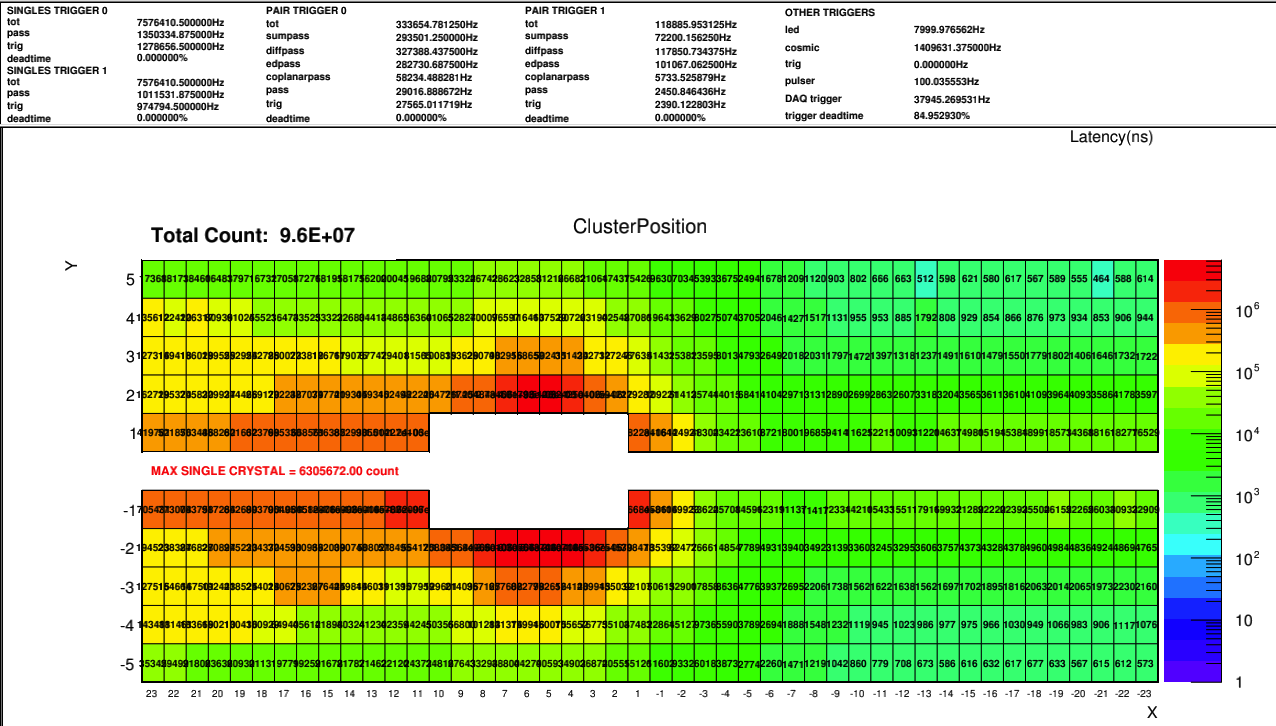
\includegraphics[width=0.9\textwidth]{pics/ecal-cluster-12-20-14.png}
\caption{ \label{DAQscalers} View of the DAQ scaler window.}
\end{figure}

\newpage
  \section{Strip Charts}
      The most import quantities to monitor with strip charts are temperature and HV current.  There are two programs to view strip charts of ECal EPICS variables.  The older StripTool shown in figure~\ref{temp2} can be started from the HPS\_EPICS gui.  The newer MyaViewer (which adds the ability to retrieve archive information), must be run locally on one of the computers in the counting room (\texttt{clonpcN}, where \texttt{N} is one of the numbers from 11 to 19).  The scripts to run it are in {\it hpsrun}'s path, so in a terminal enter one of:
      
      \begin{itemize}
          \item \texttt{mya\_ecal\_all.sh}
          \item \texttt{mya\_ecal\_temp.sh}
          \item \texttt{mya\_ecal\_curr.sh}
          \item \texttt{mya\_ecal\_voltage.sh}
      \end{itemize}

\newpage

   \section{LED Monitoring}
      \subsection{System operations}
      The LED system is operated through an EPICS GUI accessible from the main HPS EPICS menu, through Devices, then Flasher (see Figure \ref{FlasherMEDM}).

Shift takers are requested to operate the system in ``Sequence mode'' only. To do so, when requested, click on ``Initialize Flasher'', then verify the TOP frequency is 8000 Hz, and if necessary adjust it trough the proper drop-down menu. Finally, to start the sequence, click on ``Start Blue Seq'' (to use blue LEDs) or ``Start Red Seq'' (to use red LEDs). During such a run the DSC scaler screen allows to check the proper functioning of the channels (figure~\ref{LEDScalers}). 

\begin{figure}[htbp]
\center
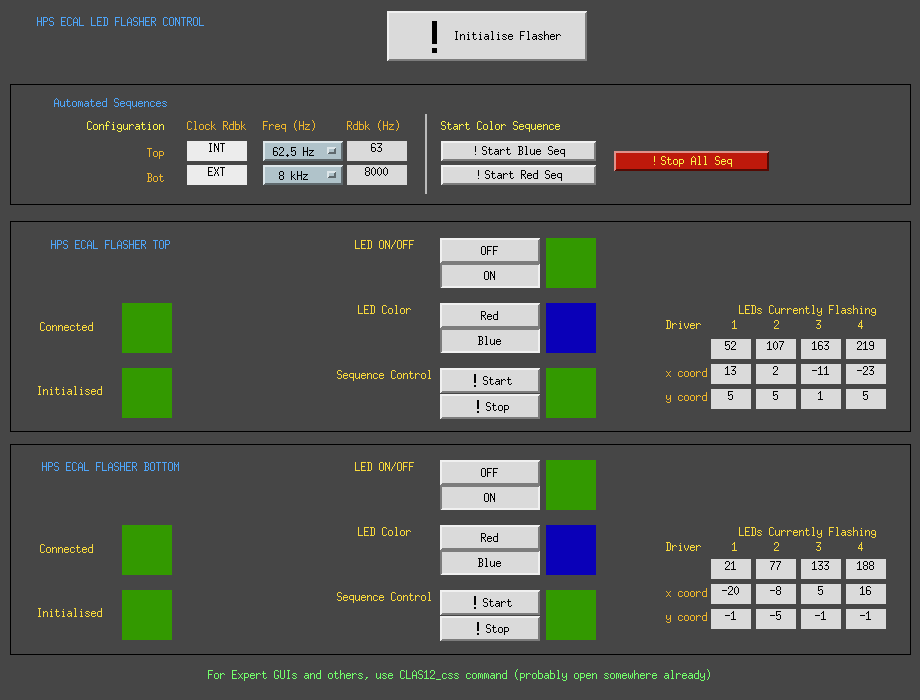
\includegraphics[width=0.75\textwidth]{pics/FlasherMEDM.png}
\caption{ \label{FlasherMEDM} The HPS-ECAL Led monitoring system EPICS GUI.}
\end{figure}
\begin{figure}[htbp]
\center
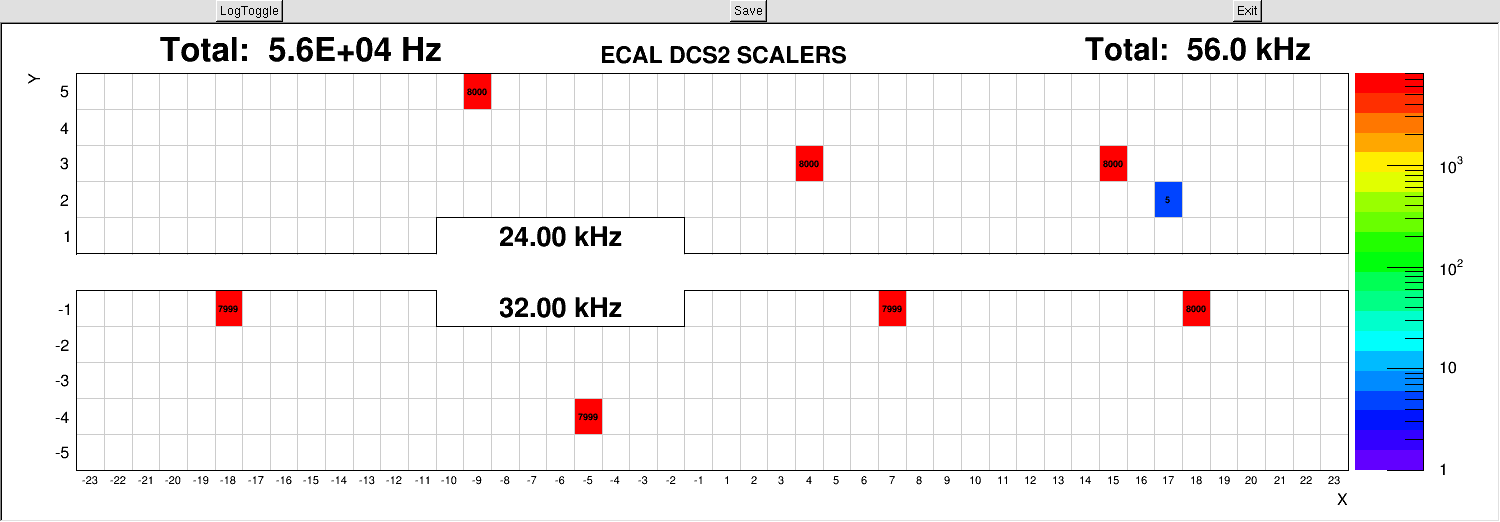
\includegraphics[width=0.95\textwidth]{pics/DSCScalersLED_2014_12_20.png}
\caption{ \label{LEDScalers} The HPS DSC scaler during a LED run.}
\end{figure}

\subsection{Automatic LED Monitoring}
A monitoring app is setup to record all channels successfully registered during an LED run.  It should be started before the LED sequence is started and viewed afterwards, with the command: \begin{center}\$HOME/hps\_software/scripts/startECalLEDSequenceMonitoring.csh\end{center} Make sure to use the hpsrun account before using this command.
  
\subsection{Taking an LED sequence run}
The following instructions must be followed to take an LED sequence run. This involves setting the DAQ, starting the LED sequence run, and configure the hps-java monitoring app to monitor the data. At the end of the run, the user can upload the relevant information to the hps conditions database, as well as post a log-entry to the HallB electronic logbook.

\subsubsection{Setup}
Follow these instructions to setup the system before takin the LED sequence run.
It is critical they are followed in the \textbf{exact} order as they are here reporter.

\begin{enumerate}
\item{\textbf{Start the DAQ system: }
\begin{itemize}
\item Identify the machine where the DAQ RunControl is running. If you can't find it anywhere, it is possible the DAQ system has to be initialized from scratch. To do so, refer to the HPS DAQ manual, or contact the DAQ expert.
\item Depending on the DAQ state, different buttons may be visible in the ``Transition'' area. If the ``Configure'' button is not visible, click on ``Reset'', then on ``OK''.
\item Click on ``Configure'' to properly set up the run.
A ``Run Type Configuration'' dialog will show up.

Use the scroll-down menu to select as RunType: HPS3ECAL\_NOER\_NOTDC. This configuration will not save any data on tape (only online analysis will be performed)

Use instead: HPS3\_ECAL\_NOTDC to save data on tape.

Then, click on ``Config'' button. A file-chooser menu will show up.

Select: /usr/clas12/release/0.2/parms/trigger/HPS $\rightarrow$ ECAL $\rightarrow$  HPS\_ECAL\_LED\_RUN.trg. 

Click on ``OK'' to close the file-choose menu.

Click on ``OK'' in the Run type dialog.

{\bf \it TODO: Update this section if DAQ configuration changes}

\item{Click on ``Download'', then on ``Prestart''.  Wait until the ``GO'' button appears, but {\bf do not click on it yet.}

 }
\end{itemize}
}
\item{\textbf{Start the monitoring app: }Use the command outlined in the previous section to start the monitoring app.

\textcolor{red}{\bf Do this after the run-control shows the ``GO'' button.}

When the main gui window shows up, click on the ``Connect button''. The Ecal event display will show up.}
\item{\textbf{Initialize the LED monitoring sequence:}In the EPICS gui, click on ``Initialise Flasher'', then on ``!Stop All Seq'' (to ensure there are no previous sequences running). 

For both controllers, ensure the LED ON/OFF button is set to OFF (RED square). If not, click on OFF.}
\end{enumerate}
      
\subsubsection{Run start, data taking, and run stop}
To start data taking follow these instructions, in the exact order they are reported here.
\begin{enumerate}
\item In the RunControl GUI, click on the ``GO'' button. Wait 10~s, until the message ``transiction go succeded'' is displayed in the log window and the ``END'' button displays. 
\item In the EPICS gui, click on ``Start Blue Seq'' or ``Start Red Seq''.

By default, take a BLUE sequence. 

Take a RED sequence only if the Ecal expert ask you to do so.
\end{enumerate}

While the LED sequence is running, you can look at the monitoring application to check data being recorded. The event display will show 8 crystals at time with a signal. A full sequence will take $\simeq$ 10 minutes to complete.

{\bf  The DAQ system is not set up to end the run when the LED sequence is completed.} When the sequence is complete:
\begin{itemize}
\item The LED system automatically turns off. As a direct consequence of this, no further triggers are sent to the DAQ system
\item The data-taking run is \textbf{not} ended. This means the DAQ will stay in RUN mode, but no events will be recorded, since there are no triggers.
\end{itemize}
{\bf
Use the EPICS gui to periodically check the sequence status, looking at the Sequence Control section (RED is OFF, GREEN is ON). Tipically, a sequence will take $\simeq$ 10 minutes to complete.}

The user can confirm the sequence has actually ended by looking at the ECal Event display: no crystals have signal when the sequence is off.

When both sequences are OFF, first turn OFF both controllers (LED ON/OFF, click on OFF), 
then use the DAQ run control to END the run, by clicking on the ``End'' button.



\subsubsection{Analysis at the run end}

When the run ends, the monitoring application automatically recognizes this, and the online analysis of the measured data starts. 

A pop-up will appear, asking the user if he wants to upload the LED data that has been measured to the HPS conditions database: uploaded quantities are the average channel response to LED pulses and the RMS. Before confirming this, the user is required to have a look at the average charge per LED, displayed in the monitoring app: tab Ecal Led Sequence, sub-tab Sequence Map. The average channel response should be in the range $\simeq 20 \div 30$. 

An automatic log entry in the Hall B logbook will also be made, with the Sequence Map image. The user is requested to complete the comment form with any relevant observation, and then click on ``OK''

{\bf {\it TODO: print a reference map and aks the user to compare with that}}

\subsection{Quick 2-Minute LED Run for Simple Channel Status Check}
{\em Note, this has become deprecated and unsupported now that we replaced splitters with
patch panels and no longer have discriminators.  Using FADCs to perform the same task is
possible but yet to be implement, since that requires reconfiguring the FADC boards'
thresholds every time and lessens the quickness and usefulness of this.}

This just counts threshold crossings in the discriminators, which is sufficient for checking that all channels are alive with LEDs.  This full test of all 442 channels requires only 2 minutes, requires no changes to the DAQ configuration, and is completetely independent of the hps-java monitoring app.  If all LEDs and all channels are working, the result should be similar to Figure~\ref{fig:quickledscanresult}

  \begin{enumerate}
      \item With a quiet detector, execute the command \texttt{runEcalLedTest.sh}.  This will open a gui showing accumulated scaler rates in all 442 ECal channels.  
      \item Start a ``LessFast'' LED sequence.
      \item Check that all channels are uniformly populated to within a factor of 2 after the sequence is finished.
  \end{enumerate}

  \begin{figure}[htbp]\centering
      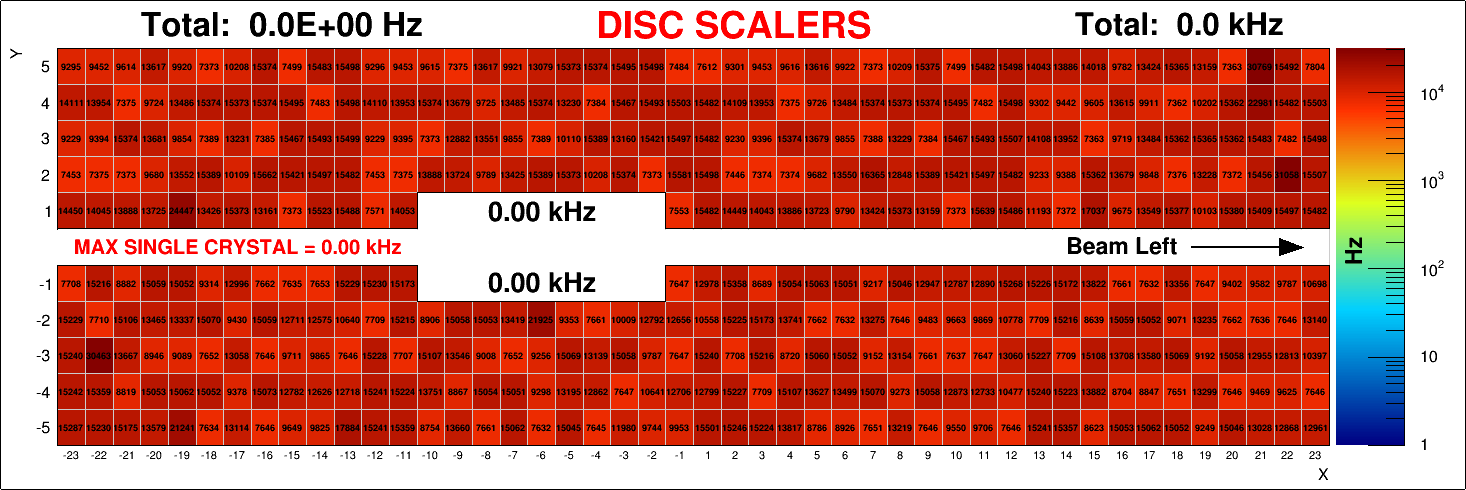
\includegraphics[width=14cm]{pics/ledScanBlue_2015_04_17_10-45-53.png}
      \caption{The accumulated discriminator counts after a successfull ``Quick 2-Minute LED Run''.  The absolulte counts will depend on LED pulser rate and duration, but the important aspect is uniformity from channel to channel.  \label{fig:quickledscanresult}}
  \end{figure}


   \section{Taking a Cosmic Calibration Run}

   In addition to the calorimeter's HV, the cosmic PMTs should be powered on.  Their HV control is under ``Cosmic PMTs'' in the ``Controls'' button of the main ECal EPICS gui's HV section (Figure ~\ref{fig:ecal_all}) and shown in Figure~\ref{fig:cosmicPMTs}.  They are named \texttt{ECal\_cosm1} and \texttt{ECal\_cosm2} and their voltages should be set at 1650 V.  The DAQ configuration should be set to \begin{center}\texttt{hps\_cosmic.trg}\end{center}.
       \begin{figure}[htbp]\centering
           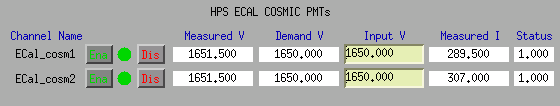
\includegraphics[width=0.8\textwidth]{pics/cosmicPMTs.png}
           \caption{Controls for PMTs for cosmic trigger.\label{fig:cosmicPMTs}}
       \end{figure}


   \section{Taking a Pedestal Run}

   Pedestals are calculated at running luminosity with DAQ configuration \begin{center}\texttt{ecalPedestal.trg}\end{center} and monitored and analyzed with HPS's hps-java monitoring app via the command:
       \begin{center}\texttt{startEcalPedestalCalculator}\end{center}
       In this monitoring app you can click on the event display to view the different channels' pedestal histograms as the data is acquired.  Once the statistics are sufficient, the app should be disconnected from the ET-ring and then output files for the DAQ and database will be generated in the directory:\begin{center}\texttt{\$HOME/EcalPedestals}\end{center}  The user will be asked if they want them put in the database automatically, and it requires two consecutive ``YES'' responses to make it happen.  An expert should make the trigger configuration use the new pedestal file.


\newpage

\part{ECal Experts Resources}

   \section{Location of ECal Elements}

   {\em{\bf REMINDER:} Since the ECal is within 3 feet of the beamline, it needs to be surveyed by RADCON before any work can be done on it.}
   {\footnotesize
\begin{itemize}
\item
The chiller is located beam-left just downstream of the calorimeter on the ground in the Alcove.
\item
The LED controllers are located at the top of the rack closest to the beamline in the Alcove.
\item
The TDCs and DISCs are are in the rack closest to the beamline in the Alcove.
\item
The FADCs and patch panels occupy the rack furthest from the beamline in the Alcove.
\item
    The HV supply is on the Pie Tower in the rack closest to the beamline.  See figure~\ref{fig:HVPHOTO}.
\item
    The LV supply is on the Pie Tower at the top of the middle rack. See figure~\ref{fig:LVPHOTO}.
\end{itemize}

\begin{figure}[htbp]\centering
    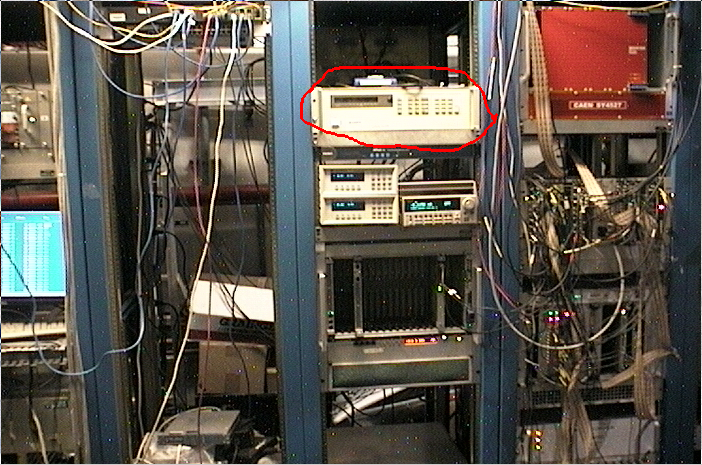
\includegraphics[width=7cm]{pics/ECALLVPHOTO2.png}
    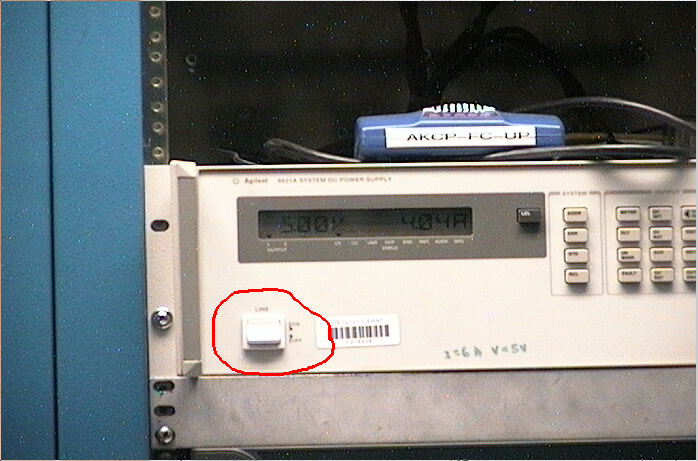
\includegraphics[width=7cm]{pics/ECALLVPHOTO.png}
    \caption{Location of Agilent LV power supply near the top of the middle rack in the pie tower.  Power switch is circled in red.\label{fig:LVPHOTO}}
\end{figure}
\begin{figure}[htbp]\centering
    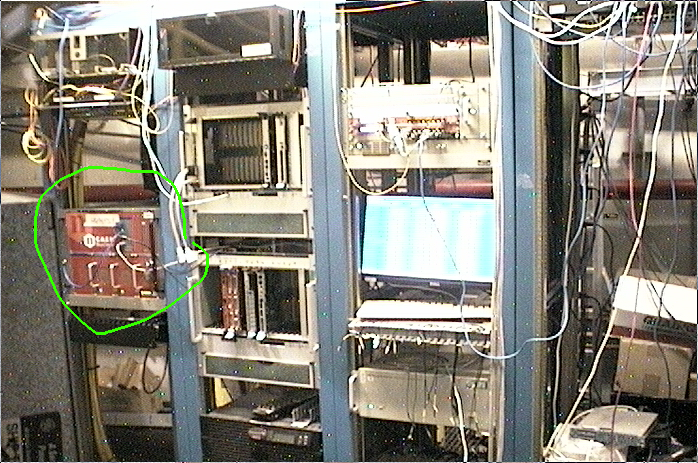
\includegraphics[width=9cm]{pics/ECALHVPHOTO.png}
    \caption{Location of the CAEN SY4527 HV power supply in the left-most rack in the pie tower.  Key for on/off is in the lower right corner of the crate.  The crate is labeled ``HVHPS2''. (The LV supply is just out of the picture to the right.)\label{fig:HVPHOTO}}
\end{figure}

\newpage
   \section{Cooling system}

   The cooling system is using an ANOVA A-40 chiller that can be controlled through EPICS (\ref{ChillerCam}). The setting should not be modified; the temperature setting should be fixed at 17 degrees Celsius.  If any of the readbacks in our EPICS screens for these systems are empty and white, it may be necessary to reboot the corresponding IOC. 
   %In case of problem with the chiller contact ??? (who can take care of these in Hall-B engineer group?).  
   %The manual for the chiller can be found here:
   %{\noindent\footnotesize\url{http://www.nist.gov/ncnr/upload/Circulating-Bath\_Thermo-Scientific\_NESLAB-RTE-7.pdf}}
     \subsection{Rebooting the Chiller After Power Failure}
     {\em This section applies to the old Thermo-Scientific chiller that was replaced in April 2015.  We have not had the opportunity to experience how the new ANOVA A-40 chiller responds to a power failure while in remote mode.}

     If the chiller loses power while in local mode, the ``power'' button must be pressed manually to restart it after power is restored.  In case it loses power while in remote mode, a procedure is necessary to reset it after power is restored:
   {\footnotesize
     \begin{enumerate}
         \item Hold the ``up'' and ``down'' arrow buttons simultaneously for 10 seconds.
         \item Press the ``computer'' button to go into local mode.
         \item Press the ``power'' button to turn it off.
         \item Press the ``power'' button to turn it on.
         \item Press the ``computer'' button to return to remote mode.
    \end{enumerate}
    }

    \subsection{Restarting the Chiller IOC}
    Chiller IOC runs in ``procserv'', a wrapper that automatically runs and restarts services and provides access to them via telnet.  To restart the chiller's IOC:
   {\footnotesize
   \begin{enumerate}
       \item \texttt{`ssh hpsrun@clonsl1'}
       \item \texttt{`softioc\_console iocchiller'} and type user's password if necessary.
       \item \texttt{`ctrl-x'} to restart the IOC
       \item \texttt{`ctrl-]'} to quit to telnet
       \item \texttt{`quit'} to exit telnet
   \end{enumerate}
   }
\noindent{\em Don't leave a terminal open connected to this telnet session.}

   \subsection{Restarting the Temperature Monitoring IOC}
   Thermocouples are used to monitor the temperature inside and outside the calorimeter.  To restart the IOC that reads these:
   {\footnotesize
   \begin{enumerate}
       \item \texttt{`ssh hpsrun@clonsl1'}
       \item \texttt{`softioc\_console ioctempSens'} and type user's password if necessary.
       \item \texttt{`ctrl-x'} to restart the IOC
       \item \texttt{`ctrl-]'} to quit to telnet
       \item \texttt{`quit'} to exit telnet
   \end{enumerate}
   }
\noindent{\em Don't leave a terminal open connected to this telnet session.}


\newpage
   \section{LV Supply}
      The low voltage power supply is an Agilent 6621.  It should be set with both channels at $+5$V with their current limits at 6 A, while external wiring inverts one channel to create a bipolar $\pm5$V supply. 

      The low voltage supply might have difficulties to get to full voltage because of high current. If that was the case check, with all power supplies off, that all connection are goods. Then contact run coordinator to see if LV power supply addition is possible. 

\subsection{Changing LV Settings}
The LV supply can be controlled via its EPICS expert screen (figure~\ref{lvexpert}), accessible from the grey button in the top right of the LV section of the main ECAL EPICS screen (figure~\ref{fig:ecal_all}). In general the only necessary changes are powering on/off, while voltage and current setpoints are never changed from 5V/6A.
\begin{figure}[htbp]\centering
    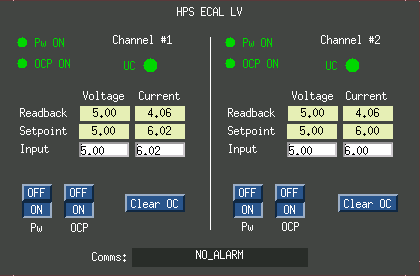
\includegraphics[width=9cm]{pics/lvexpert}
    \caption{The LV expert EPICS screen in normal operation.\label{lvexpert}}
\end{figure}

{\em Note, as a safeguard, if one currently tries to use EPICS to set the voltage greater than 5 V or the current greater than 6 A, the request will be ignored by the IOC.}  Overriding these limits can currently only be done either via local control (Section \ref{sec:lvlocalops}), or by setting new values for the limits via \texttt{caput}.  The corresponding PVs are:
\begin{itemize}
    \item\texttt{HPSECALLV:i1set:DRVH}
    \item\texttt{HPSECALLV:i2set:DRVH}
    \item\texttt{HPSECALLV:v1set:DRVH}
    \item\texttt{HPSECALLV:v2set:DRVH}
\end{itemize}

\subsubsection{Local Operation}\label{sec:lvlocalops}
The LV supply can also be controlled manually in the hall via buttons on its front panel.  However, when in remote mode (denoted by the ``RMT'' marker in its LCD display), local operations require pressing the ``LCL'' button first, then quickly pressing the desired operation button before remote mode is automatically reenabled by the IOC.  Completely disabling this ``feature'' requires stopping the IOC (see section~\ref{lviocstop}).

\newpage
\subsection{Restarting the LV IOC}
   To restart the IOC:
   {\footnotesize
   \begin{enumerate}
       \item \texttt{`ssh hpsrun@clonsl1'}
       \item \texttt{`softioc\_console iocA6621'} and type user's password if necessary.
       \item \texttt{`ctrl-x'} to restart the IOC
       \item \texttt{`ctrl-]'} to quit to telnet
       \item \texttt{`quit'} to exit telnet
   \end{enumerate}
   }
\noindent{\em Don't leave a terminal open connected to this telnet session.}

\subsection{Disabling the LV IOC}\label{lviocstop}
   To disable the IOC:
   {\footnotesize
   \begin{enumerate}
       \item \texttt{`ssh hpsrun@clonsl1'}
       \item \texttt{`softioc\_console iocA6621'} and type user's password if necessary.
       \item \texttt{`ctrl-t'} to toggle auto-restart
       \item \texttt{`ctrl-x'} to kill the IOC
       \item \texttt{`ctrl-]'} to quit to telnet
       \item \texttt{`quit'} to exit telnet
   \end{enumerate}
   }
\noindent{\em Don't leave a terminal open connected to this telnet session.}

\newpage
   \section{High Voltage}
   \subsection{Restarting the HV IOC}
   Occaissonaly the soft IOC for the HV needs to be manually restarted.  Symptoms of this condition include errors messages from EPICS when trying to turn on/off voltages and white blocks in the main HV screen (figure~\ref{HV}).  {\em Note, the IOC always needs to be restarted if the HV CAEN mainframe is power cycled.}

   To restart the IOC:
   {\footnotesize
   \begin{enumerate}
       \item \texttt{`ssh hpsrun@clonsl1'}
       \item \texttt{`softioc\_console iocecalVoltages'} and type user's password if necessary.
       \item \texttt{`ctrl-x'} to restart the IOC
       \item \texttt{`ctrl-]'} to quit to telnet
       \item \texttt{`quit'} to exit telnet
   \end{enumerate}
   }
\noindent{\em Don't leave a terminal open connected to this telnet session.}
   
   \subsection{Changing HV Settings}
      {\bf NOTE:} Changing voltage settings should be taken care of in coordination with the ECal group (contact R.~Dupre). Current setting can be increased in case of need, please document this change in the log book and notify the ECal expert on call.

 {\bf NOTE:} The ECal HV groups were renumbered for EPICS, and the correspondence map (figure~\ref{ExpertMap}) is available in the expert ECal HV monitoring window (Figure 
 \ref{HV}) via the ``Expert HV Map'' button.

\begin{figure}[htbp]
\center
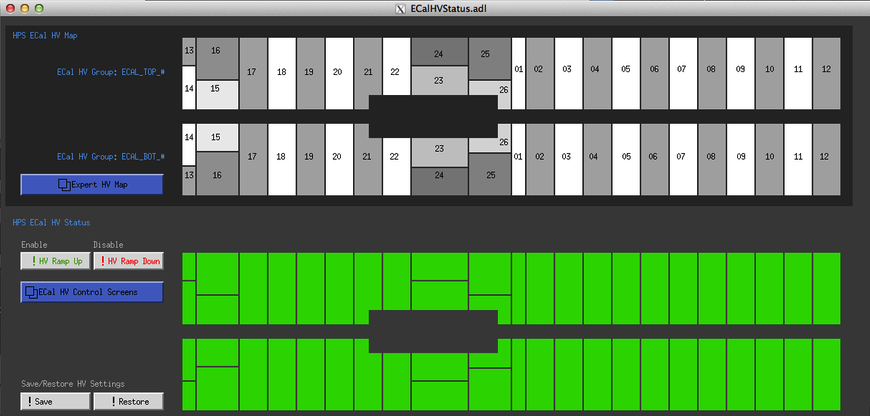
\includegraphics[width=0.95\textwidth]{pics/ecalhvmongui.png}
%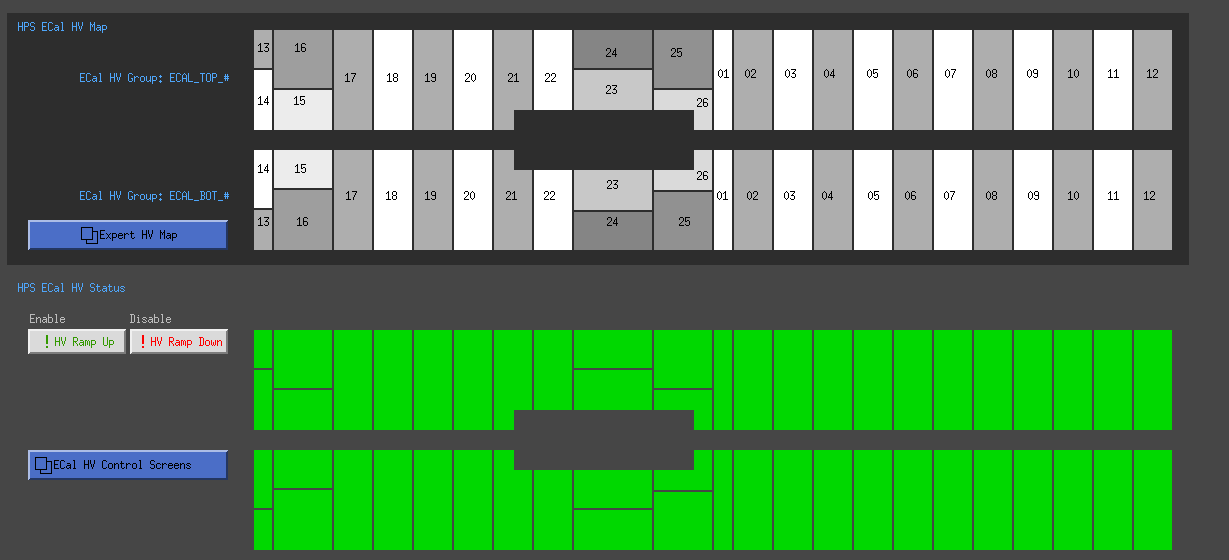
\includegraphics[width=0.95\textwidth]{pics/ecalhv_2014_12_15_16:02:54.png}
\caption{ \label{HV} View of the EPICS ECal HV expert monitoring window.}
\end{figure}

\begin{figure}[htbp]
\center
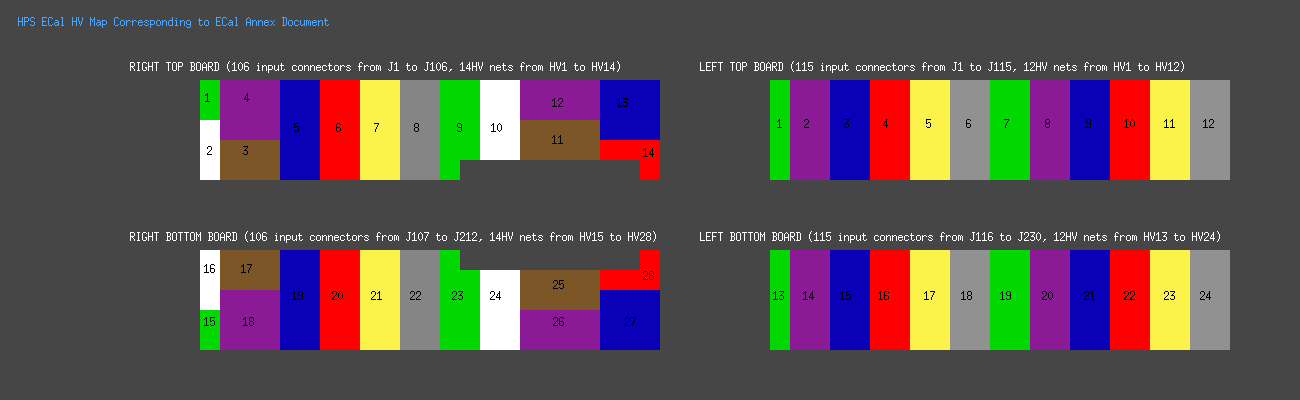
\includegraphics[width=0.95\textwidth]{pics/ecalhv_expertmap_2014_12_15.png}
\caption{ \label{ExpertMap} Expert HV channel map for reference.}
\end{figure}

      If for some reason some channels were to drop in gain (or increase) or if the current drawn increases in a group, it might be necessary to change the HV settings in the expert ECal EPICS control (Fig.~\ref{EHV}). A modification of the voltage will lead to a modification of the gain used by the trigger system, these values need to be updated at the same time!
    
      \subsubsection{HV Save/Restore}
      A system to save and restore the entire calorimeter's voltage settings is available via buttons in the ECAL HV expert window in Figure \ref{HV}.  If the voltage setpoints are changed, a backup should be made of the new settings.  This must be run as a user in group \texttt{clas-4};  user \texttt{hpsrun} does not have sufficient priveleges to save/restore voltage settings. 
      An example of the restore window is shown in figure~\ref{fig:hvrestore}, which is accessible from the HV expert screen shown in Figure~\ref{HV}.

\begin{figure}[htbp] \centering
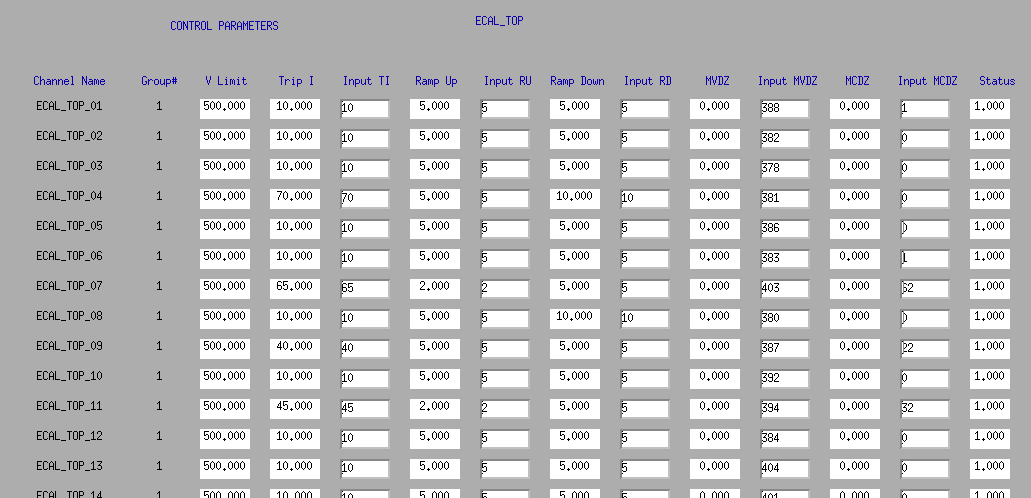
\includegraphics[width=0.85\textwidth]{pics/ecalhv_parameters_2014_12_15.png}
\caption{ \label{EHV} Cropped view of the EPICS HV expert control window. It is accessed from the parameters button in the ECal HV control screen \ref{HVControl}}
\end{figure}

\begin{figure}[htbp]\centering
    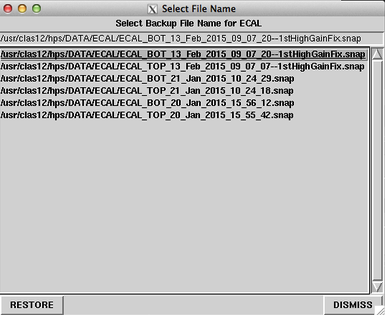
\includegraphics[width=8cm]{pics/hvrestore.png}
    \caption{The gui interface to save/restore HV settings.  \label{fig:hvrestore}}
\end{figure}

   \subsection{Long Term HV monitoring}

   An hourly snapshot of HV currents is stored by a cron job (and in the EPICs and MYA databases).  Currently the easiest way to view it is as user \texttt{hpsrun} on \texttt{clonpcNN} by excuting the command:
   \begin{center}
   \texttt{\$HOME/.ecalhv/plotEcalHV.py}
   \end{center}
The product should be a plot like figure~\ref{HVhistory}.

\begin{figure}[htbp] \centering
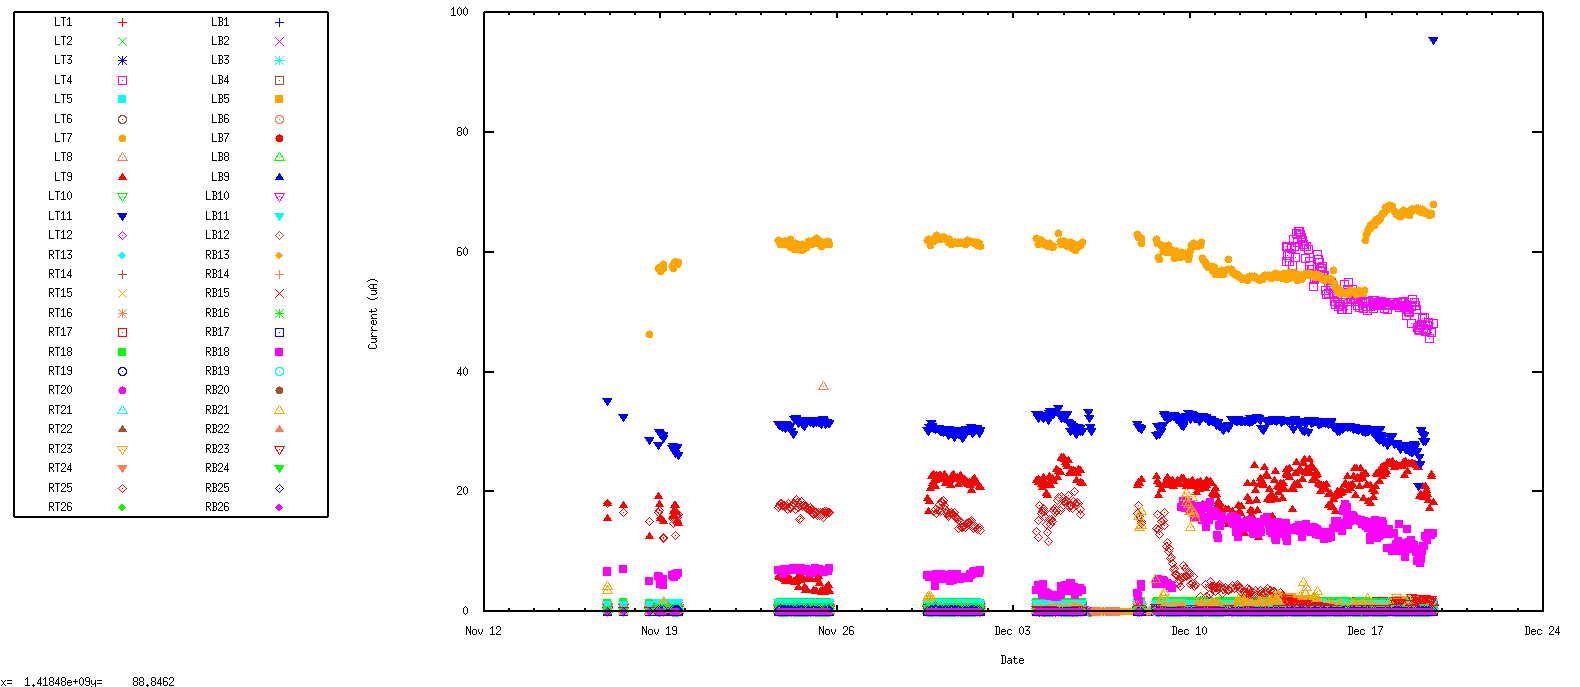
\includegraphics[width=0.95\textwidth]{pics/ECALHVCURRENTS_2014_12_20.png}
\caption{ \label{HVhistory} Expert HV current history.}
\end{figure}

\newpage
\section{Channel Mapping GUI}
Channel mapping is available in a spreadsheet in the annex pdf on the HPS Run Wiki. It is also available in an interactive GUI (shown in Figure \ref{fig:kylesGui}) which can be run by executing \begin{center}\texttt{kylesGui.sh}\end{center} in a terminal.

The user can hover over a crystal with the mouse to see all its channel numberings in the table at the bottom of the window.  This includes x/y-indices, APD and LED channel numbers, FADC slot/channel, JOUT connector and channel, and HV group.  {\em Note that preamp numbers in this GUI are no longer copmletely correct after their partial replacements prior to the 2015 Engineering Run}.  

There is also a filtering option in the {\bf View} menu to highlight all channels corresponding to certain criteria.

\begin{figure}[htbp]\centering
    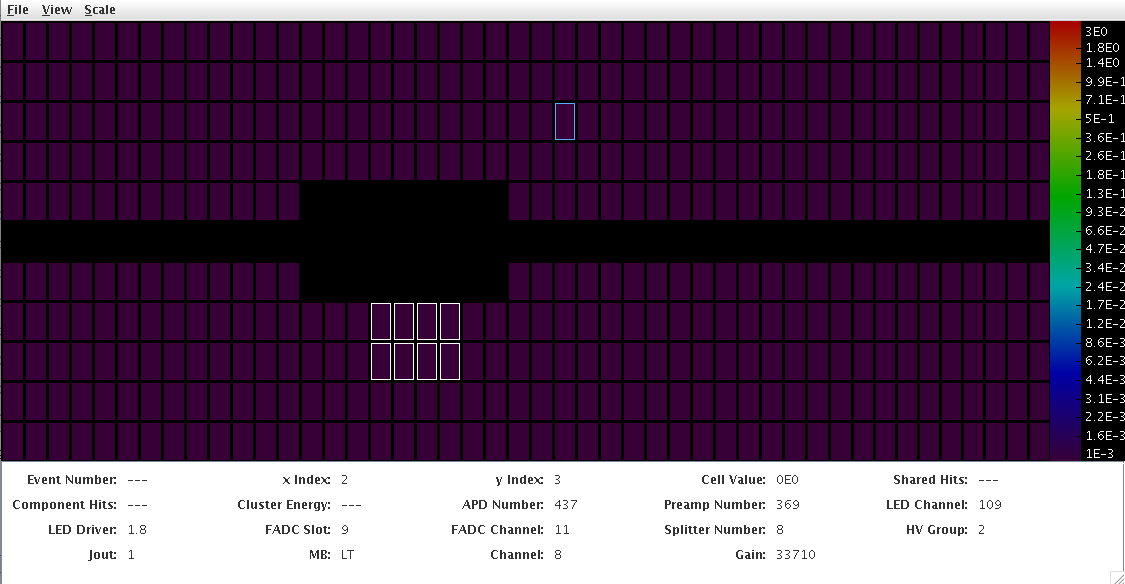
\includegraphics[width=16cm]{pics/kylesGui.png}
    \caption{The ECal event display can be used to get channel mappings.  The blue-highlighted channel's mappings are shown in the table.  The white-highlighted channels correspond to the filtering applied via the {\bf View} menu, in this case HV group 25 on bottom.\label{fig:kylesGui}}
\end{figure}

\newpage
\section{Opening the Calorimeter}

This requires 2 people.  Care must be taken for all cabling during this process, including LV, HV, signal, and thermocouples.  The required tools are shown in Table ~\ref{tab:tools}.  The blue-handled chain-winches and metric crescent wrenches should be in the HPS cabinet on the pie tower.  The rest should be retrieved from the toolboxes on the Hall-B floor.  While one can get by with only half the number of wrenches of each type, it is fastest to have the full list. 

\begin{table}[htbp]\centering
    \begin{tabular}{c|l}\hline
        Count & Type \\\hline
4&   ECAL-ONLY chain winches (blue-handled)\\
4&   15/16" crescent wrenches for rod bolts\\
2&   11 mm crescent wrenches for lateral cossbar supports (over beampipe)\\
2&   6 mm hex/allen wrenches for longitudinal crossbar supports (on far left/right)\\
2&   3/16" hex/allen wrenches for support plates\\
2&   medium-sized flathead screwdrivers\\\hline
    \end{tabular}
    \caption{Items used to open the calorimeter. \label{tab:tools}}
\end{table}

{\bf\em PLEASE return ALL tools back to where you found them.}}

   \section{Disconnection of a Channel and Preamplifier Replacement}
     
      In last resort, to recover a HV group that is tripping one can disconnect the faulty channel causing trouble. To do so, you need to find exactly which channel is involved! It might be obvious from data, if the channel was already very noisy, else you will have to test the channels of the group one by one. This is a lengthy operation and should only be attempted with the authorization of the run coordinator and in coordination with the ECal Group. It necessitates that the Hall-B crew moves the ECal out of the beam line and to open it.

   \section{LED system for experts}

This section has to be replaced with instructions to use the CLAS\_css GUI.

\begin{figure}[htbp]
\center
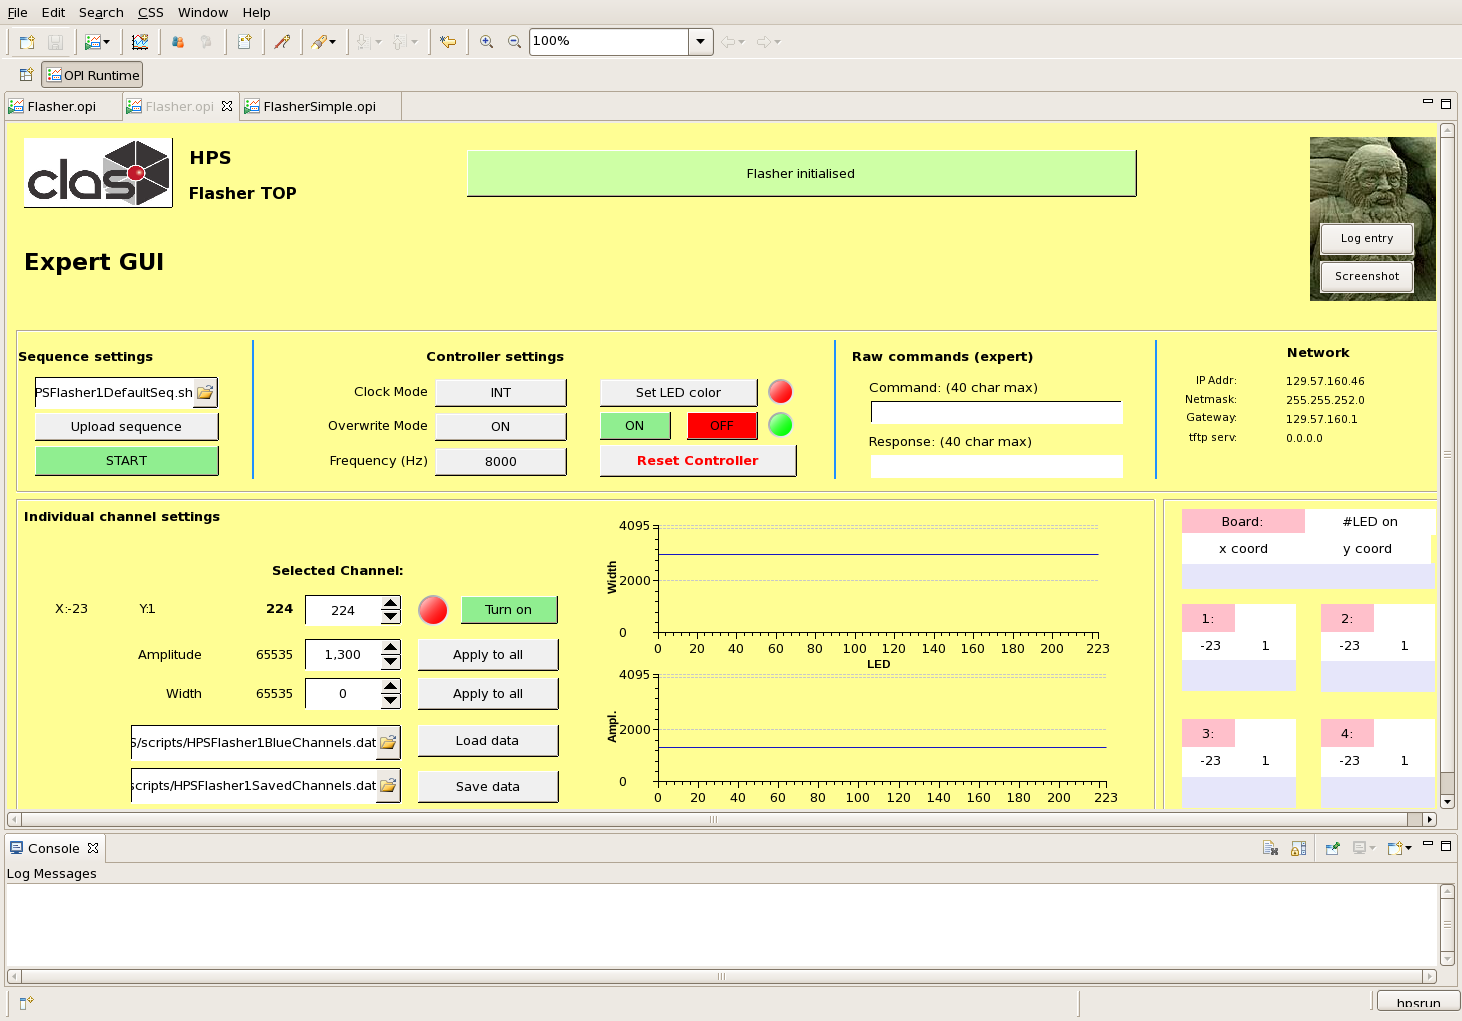
\includegraphics[width=0.85\textwidth]{pics/LEDExpert_2014_12_20.png}
\caption{\label{LEDexpert} View of the LED expert controls.}
\end{figure}

\end{document}
